\chapter{Back-Propagation}\label{backprop}

One of the most common algorithms used for deep feedforward neural network learning is the \VUname{Back-propagation} algorithm (\cite{rumelhart_learning_1986}), sometimes called \VUname{backprop}. This term is often misunderstood as meaning the whole learning algorithm, whereas in fact this name refers only to the algorithm used for computing the gradient of the network, which is then used by the actual learning algorithm, such as gradient descent (\cite{cauchy_methode_1847}), stochastic gradient descent or more advanced algorithms such as ADAM (\cite{kingma_adam:_2014}).

While backprop is commonly used for computing the gradient of a feedforward neural network, it is not limited to his task. Given a function \( f \left( \VUvec{x}, \VUvec{y} \right) \), the backprop algorithm can be used to compute the gradient of such a function with respect to \( \VUvec{x} \), i. e. \( \nabla_{\VUvec{x}} f \left( \VUvec{x}, \VUvec{y} \right) \). To use the backprop algorithm, it is useful to describe the function with a \VUname{computational graph}. A computational graph is a directed acyclic graph with nodes representing variables and edges representing operations, that is functions describing how to compute said variables. For example the equation \( y = f \left( x \right) \) is represented by two nodes, \( x \) and \( y \), and a directed edge from \( x \) to \( y \). The node representing \( y \) is labeled \( f \) as this operation can in general have multiple input variables.

\section{Chain Rule of Calculus}
\begin{theorem}\label{chain_rule}
	Let \( x \) be a real number, \( f : \VUfield{R} \to \VUfield{R} \), \( g : \VUfield{R} \to \VUfield{R} \). Let \( y = f \left( x \right) \) and \( z = g \left( y \right) \). Then
	\[ \frac{\mathrm{d} z}{\mathrm{d} x} = \frac{\mathrm{d} z}{\mathrm{d} y} \frac{\mathrm{d} y}{\mathrm{d} x} \]
\end{theorem}

This theorem can be generalized for vectors:

\begin{theorem}\label{chain_rule_vector}
	Let \( \VUvec{x} \in \VUfield{R}^n \), \( f : \VUfield{R}^n \to \VUfield{R}^m \), \( g : \VUfield{R}^m \to \VUfield{R} \). Let \( \VUvec{y} = f \left( \VUvec{x} \right) \) and \( z = g \left( \VUvec{y} \right) \). Then
	\[ \frac{\partial z}{\partial x_i} = \sum_{j = 1}^{m} \frac{\partial z}{\partial y_j} \frac{\partial y_j}{\partial x_i} \]
	or, in vector notation
	\[ \nabla_{\VUvec{x}} z = \left( \frac{\partial \VUvec{y}}{\partial \VUvec{x}} \right)^T \nabla_{\VUvec{y}} z \]
	where \( \frac{\partial \VUvec{y}}{\partial \VUvec{x}} \) is the Jacobian matrix of \( f \).
\end{theorem}

And this theorem can in turn be similarly generalized for tensors:

\begin{theorem}
	Let \( \VUmat{X} \) be a tensor, \( f \) and \( g \) functions. Let \( \VUmat{Y} = f \left( \VUmat{X} \right) \) and \( z = g \left( \VUmat{Y} \right) \). Then
	\[ \nabla_{\VUmat{X}} z = \sum_j \left( \nabla_{\VUmat{X}} Y_j \right) \frac{\partial z}{\partial Y_j} \]
	where \( j \) is a tuple of indices for \( \VUmat{Y} \).
\end{theorem}

In a computational graph, if there exists a directed edge from \( x \) to \( y \), the influence changing \( x \) has on \( y \) is represented by \( \frac{\partial y}{\partial x} \). To compute such influence between two variables which are not directly connected by an edge the chain rule can be used. This is trivial if there is only a singular directed path between the variables. Consider the following problem:

\begin{figure}[h]
	\centering
	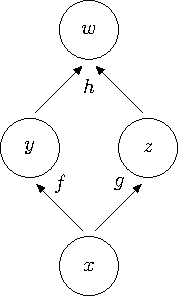
\includegraphics[width=150pt]{images/diamond/diamond.pdf}
	\caption{Diamond-style computational graph}\label{diamond}
\end{figure}

\begin{example}
	Let \( x \), \( y \), \( z \) and \( w \) be real numbers such that \( y = f \left( x \right) \), \( z = g \left( x \right) \) and \( w = h \left( y, z \right) \). The computational graph for this set of variables and operations is in figure \ref{diamond}. The derivative \( \frac{\partial w}{\partial x} \) cannot be computed directly by applying theorem \ref{chain_rule}. Instead a sum over both directed paths must be used:
	\[ \frac{\partial w}{\partial x} = \frac{\partial w}{\partial y} \frac{\partial y}{\partial x} + \frac{\partial w}{\partial z} \frac{\partial z}{\partial x} \]
	This is the result of theorem \ref{chain_rule_vector} where 
	\[ h : \VUfield R^2 \to \VUfield R : 
	\begin{pmatrix}
		y \\
		z
	\end{pmatrix} \mapsto w \]

Generally, in order to find the derivative \( \frac{\partial y}{\partial x} \) the sum of chains of partial derivatives over all directed paths from \( x \) to \( y \) must be taken. This approach becomes computationally infeasible as the number of combinations of all edges increases very quickly with the length of the path.
\end{example}
